\documentclass[border=3pt]{standalone}
\usepackage{xcolor}
\usepackage{tikz}
\usetikzlibrary{arrows.meta,decorations.pathreplacing}

\definecolor{curveblue}{HTML}{1D4ED8}
\definecolor{normalred}{HTML}{DC2626}
\definecolor{axisgray}{HTML}{64748B}

\begin{document}
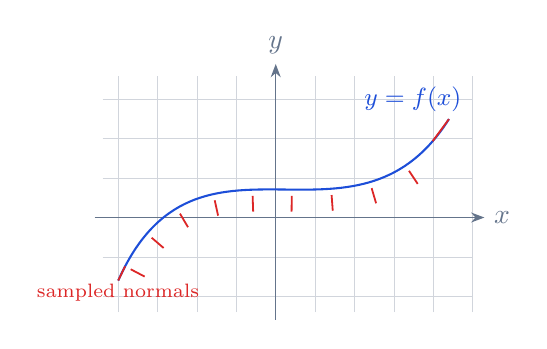
\begin{tikzpicture}[>=Stealth]
  \draw[axisgray!30,very thin] (-2.2,-1.2) grid[step=.5cm] (2.5,1.8);
  \draw[-Stealth,axisgray] (-2.3,0) -- (2.65,0) node[right] {$x$};
  \draw[-Stealth,axisgray] (0,-1.3) -- (0,1.95) node[above] {$y$};

  \draw[curveblue,line width=.75pt]
    (-2,-.8) .. controls (-1,1.45) and (1,-.65) .. (2.2,1.25);
  \draw[normalred,line width=.65pt,decorate,
    decoration={border,segment length=5mm,amplitude=2mm,angle=90,
      pre length=2mm,post length=3.5mm,mirror,raise=.8mm}]
    (-2,-.8) .. controls (-1,1.45) and (1,-.65) .. (2.2,1.25);

  \node[curveblue,anchor=west,font=\small] at (1,1.5) {$y=f(x)$};
  \node[normalred,anchor=east,font=\scriptsize] at (-.85,-.95)
    {sampled normals};
\end{tikzpicture}
\end{document}
